\hypertarget{combine-gtkdrawingarea-and-tfetextview}{%
\section{Combine GtkDrawingArea and
TfeTextView}\label{combine-gtkdrawingarea-and-tfetextview}}

Now, we will make a new application which has GtkDrawingArea and
TfeTextView in it. Its name is ``color''. If you write a name of a color
in TfeTextView and click on the \passthrough{\lstinline!run!} button,
then the color of GtkDrawingArea changes to the color given by you.

\begin{figure}
\centering
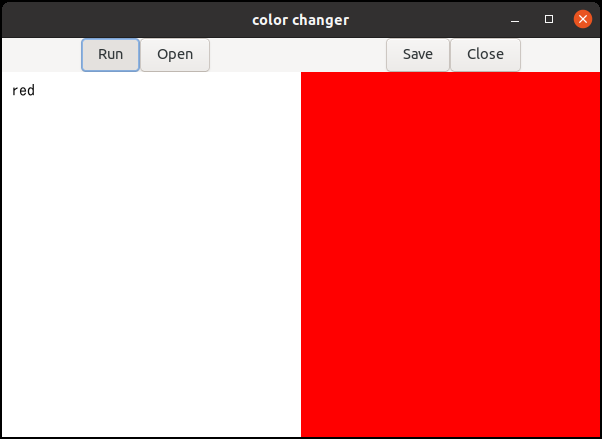
\includegraphics[width=7cm,height=5.13cm]{../image/color.png}
\caption{color}
\end{figure}

The following colors are available.

\begin{itemize}
\tightlist
\item
  white
\item
  black
\item
  red
\item
  green
\item
  blue
\end{itemize}

In addition the following two options are also available.

\begin{itemize}
\tightlist
\item
  light: Make the color of the drawing area lighter.
\item
  dark: Make the color of the drawing area darker.
\end{itemize}

This application can only do very simple things. However, it tells us
that if we add powerful parser to it, we will be able to make it more
efficient. I want to show it to you in the later section by making a
turtle graphics language like Logo program language.

In this section, we focus on how to bind the two objects.

\hypertarget{color.ui-and-color.gresource.xml}{%
\subsection{Color.ui and
color.gresource.xml}\label{color.ui-and-color.gresource.xml}}

First, We need to make the ui file of the widgets. The image in the
previous subsection gives us the structure of the widgets. Title bar,
four buttons in the tool bar and two widgets textview and drawing area.
The ui file is as follows.

\begin{lstlisting}[language=XML, numbers=left]
<?xml version="1.0" encoding="UTF-8"?>
<interface>
  <object class="GtkApplicationWindow" id="win">
    <property name="title">color changer</property>
    <property name="default-width">600</property>
    <property name="default-height">400</property>
    <child>
      <object class="GtkBox" id="boxv">
        <property name="orientation">GTK_ORIENTATION_VERTICAL</property>
        <child>
          <object class="GtkBox" id="boxh1">
            <property name="orientation">GTK_ORIENTATION_HORIZONTAL</property>
            <child>
              <object class="GtkLabel" id="dmy1">
                <property name="width-chars">10</property>
              </object>
            </child>
            <child>
              <object class="GtkButton" id="btnr">
                <property name="label">Run</property>
                <signal name="clicked" handler="run_cb"></signal>
              </object>
            </child>
            <child>
              <object class="GtkButton" id="btno">
                <property name="label">Open</property>
                <signal name="clicked" handler="open_cb"></signal>
              </object>
            </child>
            <child>
              <object class="GtkLabel" id="dmy2">
                <property name="hexpand">TRUE</property>
              </object>
            </child>
            <child>
              <object class="GtkButton" id="btns">
                <property name="label">Save</property>
                <signal name="clicked" handler="save_cb"></signal>
              </object>
            </child>
            <child>
              <object class="GtkButton" id="btnc">
                <property name="label">Close</property>
                <signal name="clicked" handler="close_cb"></signal>
              </object>
            </child>
            <child>
              <object class="GtkLabel" id="dmy3">
                <property name="width-chars">10</property>
              </object>
            </child>
          </object>
        </child>
        <child>
          <object class="GtkBox" id="boxh2">
            <property name="orientation">GTK_ORIENTATION_HORIZONTAL</property>
            <property name="homogeneous">TRUE</property>
            <child>
              <object class="GtkScrolledWindow" id="scr">
                <property name="hexpand">TRUE</property>
                <property name="vexpand">TRUE</property>
                <child>
                  <object class="TfeTextView" id="tv">
                    <property name="wrap-mode">GTK_WRAP_WORD_CHAR</property>
                  </object>
                </child>
              </object>
            </child>
            <child>
              <object class="GtkDrawingArea" id="da">
                <property name="hexpand">TRUE</property>
                <property name="vexpand">TRUE</property>
              </object>
            </child>
          </object>
        </child>
      </object>
    </child>
  </object>
</interface>
\end{lstlisting}

\begin{itemize}
\tightlist
\item
  10-53: This part is the tool bar which has four buttons,
  \passthrough{\lstinline!Run!}, \passthrough{\lstinline!Open!},
  \passthrough{\lstinline!Save!} and \passthrough{\lstinline!Close!}.
  This is similar to the toolbar of tfe text editor in Section 9. There
  are two differences. \passthrough{\lstinline!Run!} button replaces
  \passthrough{\lstinline!New!} button. A signal element is added to
  each button object. It has ``name'' attribute which is a signal name
  and ``handler'' attribute which is the name of its signal handler
  function. Options ``-WI, --export-dynamic'' CFLAG is necessary when
  you compile the application. You can achieve this by adding
  ``export\_dynamic: true'' argument to executable function in
  \passthrough{\lstinline!meson.build!}. And be careful that the handler
  must be defined without `static' class.
\item
  54-76: Puts GtkScrolledWindow and GtkDrawingArea into GtkBox. GtkBox
  has ``homogeneous property'' with TRUE value, so the two children have
  the same width in the box. TfeTextView is a child of
  GtkScrolledWindow.
\end{itemize}

The xml file for the resource compiler is almost same as before. Just
substitute ``color'' for ``tfe''.

\begin{lstlisting}[language=XML, numbers=left]
<?xml version="1.0" encoding="UTF-8"?>
<gresources>
  <gresource prefix="/com/github/ToshioCP/color">
    <file>color.ui</file>
  </gresource>
</gresources>
\end{lstlisting}

\hypertarget{tfetextview.h-tfetextview.c-and-color.h}{%
\subsection{Tfetextview.h, tfetextview.c and
color.h}\label{tfetextview.h-tfetextview.c-and-color.h}}

First two files are the same as before. Color.h just includes
tfetextview.h.

\begin{lstlisting}[language=C, numbers=left]
#include <gtk/gtk.h>

#include "../tfetextview/tfetextview.h"
\end{lstlisting}

\hypertarget{colorapplication.c}{%
\subsection{Colorapplication.c}\label{colorapplication.c}}

This is the main file. It deals with:

\begin{itemize}
\tightlist
\item
  Building widgets by GtkBuilder.
\item
  Setting a drawing function of GtkDrawingArea. And connecting a handler
  to ``resize'' signal on GtkDrawingArea.
\item
  Implementing each call back functions. Particularly,
  \passthrough{\lstinline!Run!} signal handler is the point in this
  program.
\end{itemize}

The following is \passthrough{\lstinline!colorapplication.c!}.

\begin{lstlisting}[language=C, numbers=left]
#include "color.h"

static GtkWidget *win;
static GtkWidget *tv;
static GtkWidget *da;

static cairo_surface_t *surface = NULL;

static void
run (void) {
  GtkTextBuffer *tb = gtk_text_view_get_buffer (GTK_TEXT_VIEW (tv));
  GtkTextIter start_iter;
  GtkTextIter end_iter;
  char *contents;
  cairo_t *cr;

  gtk_text_buffer_get_bounds (tb, &start_iter, &end_iter);
  contents = gtk_text_buffer_get_text (tb, &start_iter, &end_iter, FALSE);
  if (surface) {
    cr = cairo_create (surface);
    if (g_strcmp0 ("red", contents) == 0)
      cairo_set_source_rgb (cr, 1, 0, 0);
    else if (g_strcmp0 ("green", contents) == 0)
      cairo_set_source_rgb (cr, 0, 1, 0);
    else if (g_strcmp0 ("blue", contents) == 0)
      cairo_set_source_rgb (cr, 0, 0, 1);
    else if (g_strcmp0 ("white", contents) == 0)
      cairo_set_source_rgb (cr, 1, 1, 1);
    else if (g_strcmp0 ("black", contents) == 0)
      cairo_set_source_rgb (cr, 0, 0, 0);
    else if (g_strcmp0 ("light", contents) == 0)
      cairo_set_source_rgba (cr, 1, 1, 1, 0.5);
    else if (g_strcmp0 ("dark", contents) == 0)
      cairo_set_source_rgba (cr, 0, 0, 0, 0.5);
    else
      cairo_set_source_surface (cr, surface, 0, 0);
    cairo_paint (cr);
    cairo_destroy (cr);
  }
  g_free (contents);
}

void
run_cb (GtkWidget *btnr) {
  run ();
  gtk_widget_queue_draw (GTK_WIDGET (da));
}

void
open_cb (GtkWidget *btno) {
  tfe_text_view_open (TFE_TEXT_VIEW (tv), GTK_WINDOW (win));
}

void
save_cb (GtkWidget *btns) {
  tfe_text_view_save (TFE_TEXT_VIEW (tv));
}

void
close_cb (GtkWidget *btnc) {
  if (surface)
    cairo_surface_destroy (surface);
  gtk_window_destroy (GTK_WINDOW (win));
}

static void
resize_cb (GtkDrawingArea *drawing_area, int width, int height, gpointer user_data) {
  if (surface)
    cairo_surface_destroy (surface);
  surface = cairo_image_surface_create (CAIRO_FORMAT_ARGB32, width, height);
  run ();
}

static void
draw_func (GtkDrawingArea *drawing_area, cairo_t *cr, int width, int height, gpointer user_data) {
  if (surface) {
    cairo_set_source_surface (cr, surface, 0, 0);
    cairo_paint (cr);
  }
}

static void
app_activate (GApplication *application) {
  gtk_widget_show (win);
}

static void
app_startup (GApplication *application) {
  GtkApplication *app = GTK_APPLICATION (application);
  GtkBuilder *build;

  build = gtk_builder_new_from_resource ("/com/github/ToshioCP/color/color.ui");
  win = GTK_WIDGET (gtk_builder_get_object (build, "win"));
  gtk_window_set_application (GTK_WINDOW (win), app);
  tv = GTK_WIDGET (gtk_builder_get_object (build, "tv"));
  da = GTK_WIDGET (gtk_builder_get_object (build, "da"));
  g_object_unref(build);
  g_signal_connect (GTK_DRAWING_AREA (da), "resize", G_CALLBACK (resize_cb), NULL);
  gtk_drawing_area_set_draw_func (GTK_DRAWING_AREA (da), draw_func, NULL, NULL);

GdkDisplay *display;

  display = gtk_widget_get_display (GTK_WIDGET (win));
  GtkCssProvider *provider = gtk_css_provider_new ();
  gtk_css_provider_load_from_data (provider, "textview {padding: 10px; font-family: monospace; font-size: 12pt;}", -1);
  gtk_style_context_add_provider_for_display (display, GTK_STYLE_PROVIDER (provider), GTK_STYLE_PROVIDER_PRIORITY_USER);
}

#define APPLICATION_ID "com.github.ToshioCP.color"

int
main (int argc, char **argv) {
  GtkApplication *app;
  int stat;

  app = gtk_application_new (APPLICATION_ID, G_APPLICATION_FLAGS_NONE);

  g_signal_connect (app, "startup", G_CALLBACK (app_startup), NULL);
  g_signal_connect (app, "activate", G_CALLBACK (app_activate), NULL);

  stat =g_application_run (G_APPLICATION (app), argc, argv);
  g_object_unref (app);
  return stat;
}
\end{lstlisting}

\begin{itemize}
\tightlist
\item
  109-124: The function \passthrough{\lstinline!main!} is almost same as
  before but there are some differences. The application ID is
  ``com.github.ToshioCP.color''.
  \passthrough{\lstinline!G\_APPLICATION\_FLAGS\_NONE!} is specified so
  no open signal handler is necessary.
\item
  87-107: Startup handler.
\item
  92-97: Builds widgets. The pointers of the top window, TfeTextView and
  GtkDrawingArea objects are stored to static variables
  \passthrough{\lstinline!win!}, \passthrough{\lstinline!tv!} and
  \passthrough{\lstinline!da!} respectively. This is because these
  objects are often used in handlers. They never be rewritten so they're
  thread safe.
\item
  98: connects ``resize'' signal and the handler.
\item
  99: sets the drawing function.
\item
  82-85: Activate handler, which just shows the widgets.
\item
  74-80: The drawing function. It just copies
  \passthrough{\lstinline!surface!} to destination.
\item
  66-72: Resize handler. Re-creates the surface to fit its width and
  height for the drawing area and paints by calling the function
  \passthrough{\lstinline!run!}.
\item
  59-64: Close handler. It destroys \passthrough{\lstinline!surface!} if
  it exists. Then it destroys the top-level window and quits the
  application.
\item
  49-57: Open and save handler. They just call the corresponding
  functions of TfeTextView.
\item
  43-47: Run handler. It calls run function to paint the surface. After
  that \passthrough{\lstinline!gtk\_widget\_queue\_draw!} is called.
  This function adds the widget (GtkDrawingArea) to the queue to be
  redrawn. It is important to know that the window is redrawn whenever
  it is necessary. For example, when another window is moved and
  uncovers part of the widget, or when the window containing it is
  resized. But repainting \passthrough{\lstinline!surface!} is not
  automatically notified to gtk. Therefore, you need to call
  \passthrough{\lstinline!gtk\_widget\_queue\_draw!} to redraw the
  widget.
\item
  9-41: Run function paints the surface. First, it gets the contents of
  GtkTextBuffer. Then it compares it to ``red'', ``green'' and so on. If
  it matches the color, then the surface is painted the color. If it
  matches ``light'' or ``dark'', then the color of the surface is
  lightened or darkened respectively. Alpha channel is used.
\end{itemize}

\hypertarget{meson.build}{%
\subsection{Meson.build}\label{meson.build}}

This file is almost same as before. An argument ``export\_dynamic:
true'' is added to executable function.

\begin{lstlisting}[numbers=left]
project('color', 'c')

gtkdep = dependency('gtk4')

gnome=import('gnome')
resources = gnome.compile_resources('resources','color.gresource.xml')

sourcefiles=files('colorapplication.c', '../tfetextview/tfetextview.c')

executable('color', sourcefiles, resources, dependencies: gtkdep, export_dynamic: true)
\end{lstlisting}

\hypertarget{compile-and-execute-it}{%
\subsection{Compile and execute it}\label{compile-and-execute-it}}

First you need to export some variables (refer to Section 2) if you've
installed Gtk4 from the source. If you've installed Gtk4 from the
distribution packages, you don't need to do this.

\begin{lstlisting}
$ . env.sh
\end{lstlisting}

Then type the following to compile it.

\begin{lstlisting}
$ meson _build
$ ninja -C _build
\end{lstlisting}

The application is made in \passthrough{\lstinline!\_build!} directory.
Type the following to execute it.

\begin{lstlisting}
$ _build/color
\end{lstlisting}

Type ``red'', ``green'', ``blue'', ``white'', black``,''light" or
``dark'' in the TfeTextView. Then, click on
\passthrough{\lstinline!Run!} button. Make sure the color of
GtkDrawingArea changes.

In this program TfeTextView is used to change the color. You can use
buttons or menus instead of textview. Probably it is more appropriate.
Using textview is unnatural. It is a good practice to make such
application by yourself.
